% Figure: a configuration of a chain of six sites split by a region X = {2, 3}. Transcription
% (for cheap agents): six sites 0..5 on a line, each carrying a letter of the alphabet {0, 1}
% written in a small box above the site: s = (1, 0, 0, 1, 1, 0); the region X = {2, 3} is a
% dashed box around sites 2 and 3; the part on X, s|_X = (0, 1), is shaded blue; the part off X,
% (1, 0, ., ., 1, 0), is left white. Below, a second configuration s' = (1, 0, 1, 1, 1, 0) with the
% same letters off X and different letters on X, labelled "s ~_X s'" and "s' = (xi, s|_{X^c}) with
% xi = (1, 1)". The caption explains that a matrix local to X has an entry at (s, s') only when
% the two configurations agree off X, and that the entry depends on the shaded parts alone.
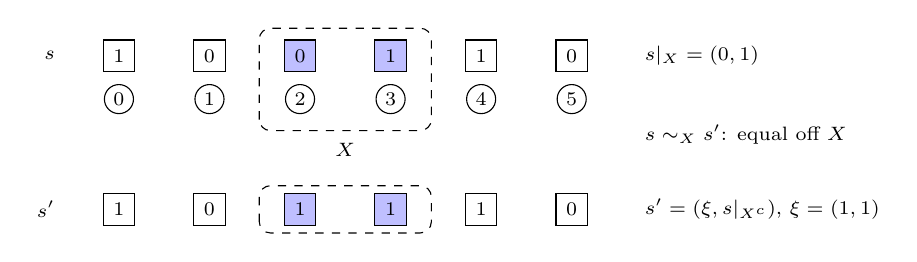
\begin{tikzpicture}[x=1.15cm,y=1cm,
  site/.style={circle,draw,fill=white,inner sep=1.6pt,font=\scriptsize},
  letter/.style={draw,rectangle,inner sep=2pt,minimum size=0.4cm,font=\scriptsize},
  onX/.style={draw,rectangle,inner sep=2pt,minimum size=0.4cm,font=\scriptsize,fill=Blue!25},
  region/.style={rounded corners=4pt,draw,dashed,fill=none},
  lab/.style={font=\scriptsize}]
  % configuration s
  \node[lab,anchor=east] at (-0.6,0.55) {$s$};
  \foreach \u/\l in {0/1,1/0,4/1,5/0} { \node[letter] at (\u,0.55) {\l}; }
  \node[onX] at (2,0.55) {0}; \node[onX] at (3,0.55) {1};
  \foreach \u in {0,...,5} { \node[site] at (\u,0) {\u}; }
  \draw[region] (1.55,-0.4) rectangle (3.45,0.9);
  \node[lab] at (2.5,-0.65) {$X$};
  % configuration s'
  \node[lab,anchor=east] at (-0.6,-1.4) {$s'$};
  \foreach \u/\l in {0/1,1/0,4/1,5/0} { \node[letter] at (\u,-1.4) {\l}; }
  \node[onX] at (2,-1.4) {1}; \node[onX] at (3,-1.4) {1};
  \draw[region] (1.55,-1.7) rectangle (3.45,-1.1);
  \node[lab,anchor=west] at (5.7,0.55) {$s|_X=(0,1)$};
  \node[lab,anchor=west] at (5.7,-1.4) {$s'=(\xi,s|_{X^c})$, $\xi=(1,1)$};
  \node[lab,anchor=west] at (5.7,-0.45) {$s\sim_Xs'$: equal off $X$};
\end{tikzpicture}
